\documentclass[a4paper,10pt,usenames]{article}
%\documentclass[color=pdftex]{beamer}
\usepackage[T2A]{fontenc}
\usepackage[utf8x]{inputenc}
\usepackage{ucs}
\usepackage{cmap}
\usepackage[english,russian]{babel}
\usepackage{amsmath}
\usepackage{graphicx}
\usepackage{indentfirst}
\usepackage{ucs} 
\usepackage[utf8x]{inputenc}
\usepackage{caption}
\usepackage{placeins}
\usepackage{listings}
\usepackage{hyperref}
\usepackage[usenames,dvipsnames]{color}    
\lstset{ 
  language=R,                     % the language of the code
  basicstyle=\small\ttfamily, % the size of the fonts that are used for the code
  numbers=left,                   % where to put the line-numbers
  numberstyle=\small\color{Blue},  % the style that is used for the line-numbers
  stepnumber=1,                   % the step between two line-numbers. If it's 1, each line
                                  % will be numbered
  numbersep=5pt,                  % how far the line-numbers are from the code
  backgroundcolor=\color{white},  % choose the background color. You must add \usepackage{color}
  showspaces=false,               % show spaces adding particular underscores
  showstringspaces=false,         % underline spaces within strings
  showtabs=false,                 % show tabs within strings adding particular underscores
  frame=single,                   % adds a frame around the code
  rulecolor=\color{black},        % if not set, the frame-color may be changed on line-breaks within not-black text (e.g. commens (green here))
  tabsize=2,                      % sets default tabsize to 2 spaces
  captionpos=b,                   % sets the caption-position to bottom
  breaklines=true,                % sets automatic line breaking
  breakatwhitespace=false,        % sets if automatic breaks should only happen at whitespace
  keywordstyle=\color{RoyalBlue},      % keyword style
  commentstyle=\color{YellowGreen},   % comment style
  stringstyle=\color{ForestGreen}      % string literal style
} 


\title{Исследование спайкового кода}
\author{Чернышев Алексей}
\setlength{\parindent}{1cm}
\def\la{\left\langle\rule{0pt}{3em}}
\def\ra{\right\rangle}
\newcommand{\HRule}{\rule{\linewidth}{0.5mm}}



\begin{document}

{ \huge \bfseries Исследование спайкового кода \\[0.4cm] }


\tableofcontents
\clearpage
\section{Спайковый код}
\indent Спайк - элементарная единица информации, которой обмениваются биологические нейроны. Соединённые синаптическими связями, нейроны, сложно и нелинейно перерабатывая вход с синапсов, вырабатывают на своём выходе (аксон нейрона), короткие электрохимические импульсы. В анализе удобно рассматривать спайки, как бинарные события (рис. \ref{spiking_neuron_pic}). 
\begin{figure}[ht]
\centering
\captionsetup{justification=centering,margin=1cm}
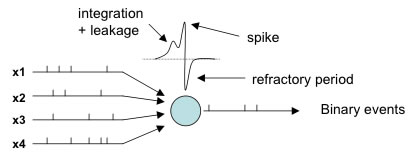
\includegraphics[width=75mm,scale=0.7]{spiking_neuron.jpg}
\caption{Спайковый нейрон}
\label{spiking_neuron_pic}
\end{figure}\\
\indent То как нейроны кодируют информацию в спайках, очень живой и трепещущий вопрос для современного научного сообщества. Важный нюанс спайкового кода в том, что он не надёжен. Исследования показали, что на один и тот же стимул популяция нейронов может дать разный ответ, что даёт огромное пространство для интерпретаций. \\
\indent На протяжении 20-ого века большинство нейрофизиологов было убеждено, что ненадёжность разрешается, если усреднять спайки на некотором промежутке времени (около 100 мс), и вся информация хранится в средних активностях нейронов. Однако, в конце 20-ого века было проведено множество исследований, показавших, что достаточно много информации хранится в самих временах спайков, и что усреднение, только ухудшает декодирование информации полученной от нейронов.\\
\indent В данном задании будет возможность закодировать сигнал в виде спайкового кода, через симуляцию популяции нейронов. Получив ответ в виде спайков, мы его декодируем, и необходимо будет сделать анализ полученных результатов, при помощи инструментов данных в этом руководстве.\\
\section{Спайковый нейрон}
\indent На рис. \ref{spiking_neuron_pic}, также, показан типичный профиль активности нейрона, основные свойство которого: 
\begin{itemize}
\item интеграция входного сигнала (integration);
\item угасание этого сигнала на нейроне со временем, или иначе говоря ``утечка'' (leakage);
\item рефракторный период, нейрон переживает его после выработки спайка, как следствие сложных химических реакций, некоторое время (от 2-10 мс) неработоспособен.
\end{itemize}
\indent Моделирование спайковых нейронов в виде наиболее приближенном к биологии, насколько позволяет современная нейронаука, возможно, но очень трудозатратно с точки зрения ресурсов компьютера. Существует модели, более менее, приближенные к биологическому аналогу и которые не так сложно моделировать. Две из них будут рассмотрены в задании.
\subsection{Модель Integrate-and-fire}
\indent Самая простая спайковая модель, основанная на RC цепи, записывается в виде дифференциального уравнения
   \begin{equation}\label{eq:iaf}
   \tau_{m}\frac{du}{dt} =-u+R I(t),
   \end{equation}
при $u \geq \vartheta$ потенциал мембраны сбрасывается и на $\tau_{ref}$ держится в сброшенном состоянии
   \begin{equation}\label{eq:iaf_reset}
   u \leftarrow u_{r} \mbox{ в течении }\tau_{ref}, 
   \end{equation}
   где $\vartheta$ - порог напряжения, временная константа мембраны $\tau_{m}=RC$, $R$ и $C$ - сопротивление и ёмкость RC-цепи соответственно, $\tau_{ref}$ - рефракторное время, $I(t)$ - приложенный ток извне, $u_{r}$ - константа описывающая потенциал мембраны покоя нейрона.\\
   \indent Пример работы такого нейрона можно посмотреть на рис.\ref{iaf_neuron_pic}.\\
\begin{figure}[ht]
\centering
\captionsetup{justification=centering,margin=1cm}
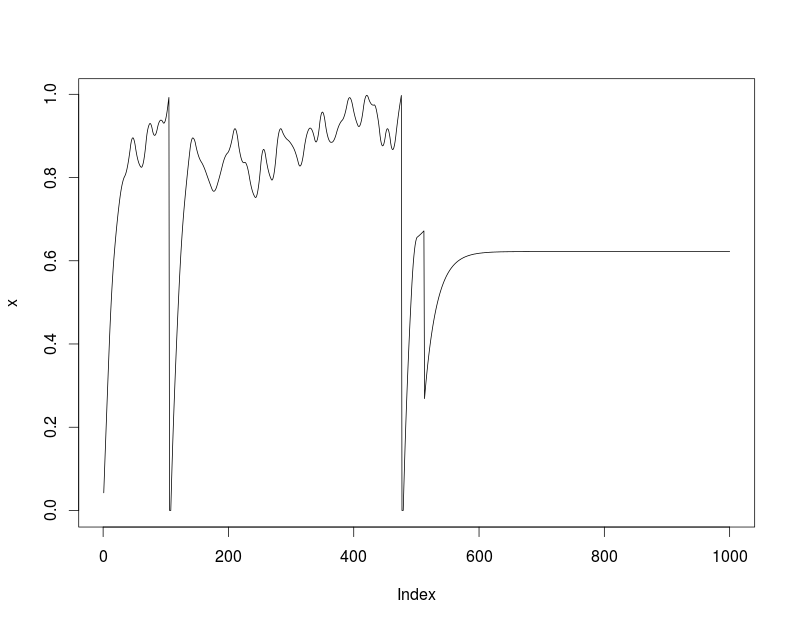
\includegraphics[width=120mm,scale=1]{iaf_profile.png}
\caption{Напряжение на мембране IaF, при $u_{r} = 0, \vartheta = 1, \tau_{ref} = 2$ мс, $\tau_{m} = 20$ мс}
\label{iaf_neuron_pic}
\end{figure}\\

\section{Пример: кодирование временного ряда}
\indent В качестве среды используется пакет \textbf{R}. Также используется набор скриптов для симуляции нейронов, его можно взять из репозитория:\\ 
\url{https://github.com/alexeyche/spike_code_project.git} \\ 
\indent Возьмём временной ряд из набора \textit{synthetic control} и нормируем его в пределах $[-1,1]$:

\begin{lstlisting}
> X = loadMatrix("~/ts/synthetic_control/synthetic_control_TRAIN_120",1)[1,]
> X =  2*(X-min(X))/(max(X)-min(X))-1
> plot(X, type="l")
\end{lstlisting}

\begin{figure}[ht]
\centering
\captionsetup{justification=centering,margin=1cm}
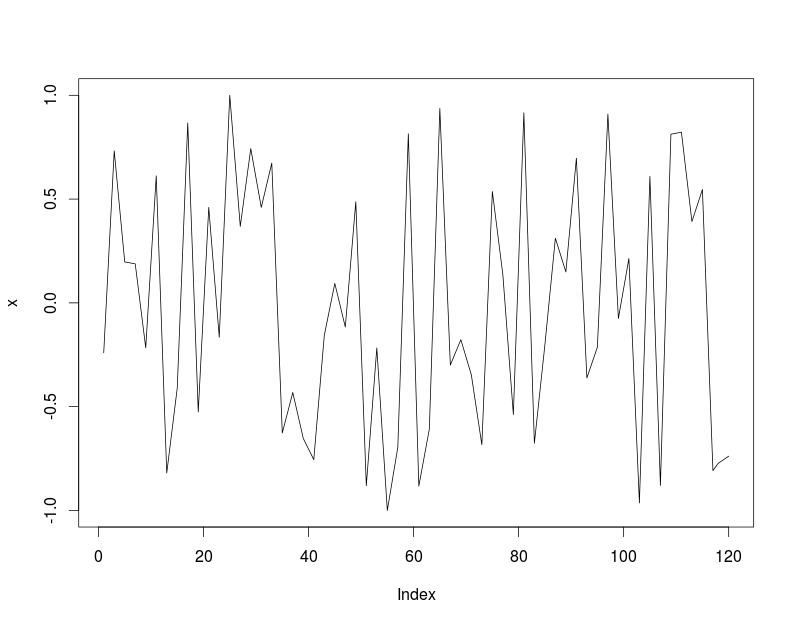
\includegraphics[width=120mm,scale=1]{synthetic_control.png}
\caption{Временной ряд}
\label{synth_control}
\end{figure}
Приложение $I(t)$ к каждому нейрону будет происходить в виде
\begin{equation}
I_{i}(t) = g_{i}X + b_{i}
\end{equation} 
где $g_{i}$ и $b_{i}$ усиление и смещение, которое для каждого нейрона уникально.\\
\indent Используя данный набор скриптов можно сгенерировать усиление и смещение для каждого нейрона, таким образом чтобы обеспечить равномерный охват сигнала $X$
\clearpage
\begin{lstlisting}
> rate_low = 0 # Herz
> rate_high = 50 # Herz
> M = 25 # Size of neuron population
> c(gain, bias) := generate_gain_and_bias(M, rate_low, rate_high)
> gain
 [1] 0.6758357 1.7004524 0.2071122 0.2756547 0.4887354 1.6412549 0.3116990 0.7759411 0.6372584 2.2066023
[11] 0.3249702 1.4093830 0.4640132 0.8744656 0.3372742 0.6675960 1.9251885 4.0983182 0.9741277 0.1989673
[21] 0.7413383 0.2470770 2.1391720 0.1389673 0.4076056
> bias
 [1]  0.76748365 -0.08399640  1.15624594  1.19207789  0.93562484  0.02672873  1.16662126  0.47109941
 [9]  0.76147893 -0.76017726  1.02079654  0.09442703  0.83244672  0.75302014  0.94207371  0.87191443
[17] -0.46682617 -2.50856272  0.54474359  1.11589300  0.91945595  0.94598459 -0.54479961  1.09119150
[25]  1.21586165
\end{lstlisting}
\indent Также распределим ответственность для каждого нейрона, за отрицательную и положительную часть графика, сгенерировав равномерное распределение из набора $\{-1,1\}$\\
\begin{lstlisting}
> encoder = sample(c(1,-1),M, replace=TRUE)
> encoder 
 [1] -1  1 -1  1 -1 -1  1  1 -1  1 -1 -1  1  1  1  1  1  1 -1  1  1 -1  1  1  1
\end{lstlisting}
\indent После всех подготовок, можно создать список с переменными для каждого нейрона, взять первую точку временного ряда, и прогнать его через популяцию $IaF$ нейронов, с характеристиками, как на рис.\ref{iaf_neuron_pic}
\begin{lstlisting}
> n = list(v=rep(0, M), ref=rep(0,M))
> input = X[1] * encoder * gain + bias
> c(n, current_spikes) := run_neurons(input, n)
> current_spikes
 [1] FALSE FALSE FALSE FALSE FALSE FALSE FALSE FALSE FALSE  TRUE FALSE FALSE FALSE FALSE  TRUE FALSE FALSE
[18] FALSE FALSE  TRUE FALSE FALSE FALSE FALSE FALSE FALSE FALSE FALSE FALSE FALSE FALSE FALSE FALSE FALSE
[35] FALSE FALSE FALSE FALSE FALSE FALSE FALSE FALSE FALSE FALSE FALSE FALSE FALSE FALSE FALSE FALSE
> which(current_spikes)
[1] 10 15 20
\end{lstlisting}
\textit{current\char`_spikes} содержит вектор булевских значений, каждое значение, отвечает за то издал спайк этот нейрон или нет
\clearpage
Прогнав цикл по всем точкам
\begin{lstlisting}
spikes = NULL
for(i in 1:length(X)) {
    x = X[i]
    input = x * encoder * gain + bias
    
    c(n, current_spikes) := run_neurons(input, n)
    spikes = cbind(spikes, as.integer(current_spikes))    
}
\end{lstlisting}
мы получим матрицу 25x120, значения которой будут говорить о том, издал ли данный нейрон в данный момент спайк или нет
\begin{lstlisting}
> gr_pl(t(spikes))
\end{lstlisting}
\begin{figure}[ht]
\centering
\captionsetup{justification=centering,margin=1cm}
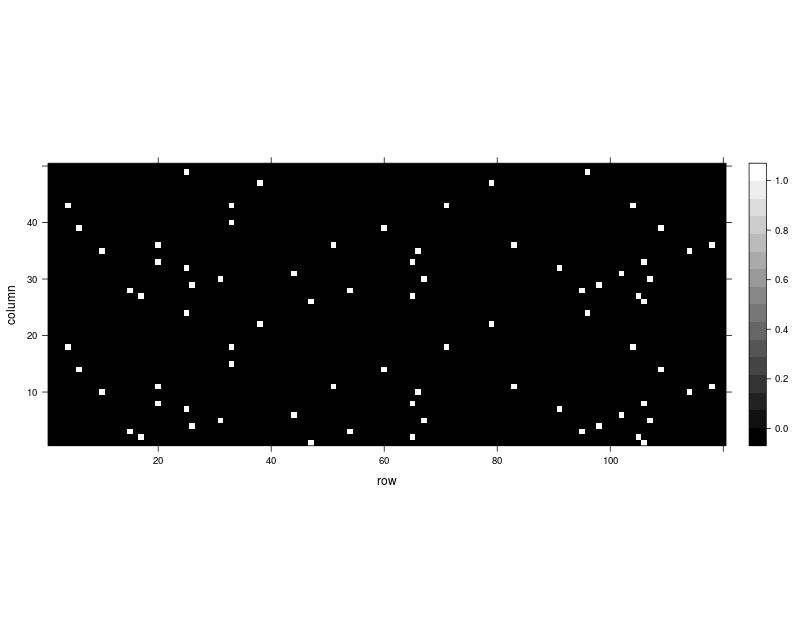
\includegraphics[width=120mm,scale=1]{rastr_plot.png}
\caption{Контурный график спайков}
\label{rastr}
\end{figure}

\end{document}
